To examine the influence of fundamental risk group dynamics on epidemics, we first
compared equilibrium prevalence and incidence using models with and without:
heterogeneity in risk,
population growth, and
risk group turnover.
We then examined the influence of different rates of turnover on
overall and group-specific equilibrium prevalence and incidence.
Finally, we examine the influence of turnover on the contribution of the
highest risk group to the overall epidemic -- as measured by the
transmission population attributable fraction (TPAF).
%% SM: suggest framing these as objective questions using precise verbs (like examine, determine, test, etc.)
%%  rather than 'to highlight, etc' as that suggests description and not an experiment.
%%  also, use one terminology consistently throughout - e.g. turnover - rather than several.
%%  In the intro, you can introduce the various ways people have conceptualized this,
%%  but in general, good to use consistent and single terminology throughout to help the reader
%%  i.e. use either 'turnover' or 'risk group dynamics', etc. but not both after introduction.
%% i find turnover easier to conceptualize; less words; and also restricts the use of term 'dynamics' in
%% reference to the epidemic dynamics, and not something else
%% JK: Agreed -- I was just using risk group dynamics to include both turnover and the other
%% two factors we briefly explore: number of risk groups & population growth. Thoughts?
% ==================================================================================================
\subsection{Model \& Simulations}\label{ss:model-sim}
We developed a deterministic single-sex SIR model
which simulates transmission in a population with heterogeneity in risk.
The model is not representative of a specific infection
%% SS: I think it might be easier to follow if it did.
%% I think it could be used as an example to thread across
%% and then in the discussion go into how this would be similar/different for another infection
%% (which parameters would likely change,
%% whether we would anticipate that the impact of turnover would be similar, different)
but includes balancing contacts
as per sexually transmitted infections \citep{Garnett1994}.
The model includes three health states:
susceptible~$\mathcal{S}$, infectious~$\mathcal{I}$, and recovered~$\mathcal{R}$
(Figure~\ref{fig:health-states}),
and $G = 3$ levels of risk:
high~$H$, medium~$M$, and low~$L$.
Risk strata are defined by different number of contacts per unit time
so that individuals in risk group $i$ are assumed to
form contacts at a rate $C_{i}$.
The probability $\rho_{ik}$ of contact formation between individuals in group $i$
with individuals in risk group $k$ is assumed to be
proportionate to the total number of available contacts within each group:
\begin{equation}
  \rho_{ik} = \frac
    {C_k x_k}
    {\sum_{\mathrm{k}}C_{\mathrm{k}} x_{\mathrm{k}}}
    \label{eq:rho}
\end{equation}
\begin{figure}
  \centering
  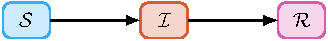
\includegraphics[width=0.4\linewidth]{health-states}
  \caption{Modelled health states.
  $\mathcal{S}$: susceptible;
  $\mathcal{I}$: infected;
  $\mathcal{R}$: recovered;
  $\lambda$: force of infection;
  $\tau$: treatment.}
  \label{fig:health-states}
\end{figure}
\par
The biological probability of transmission is defined as $\beta$ per contact.
Individuals transition from the
infectious $\mathcal{I}$ to susceptible $\mathcal{S}$ health-state
via a force of infection $\lambda$ per year, per susceptible in risk group $i$:
\begin{equation}
  \lambda_{i} =
  C_{i} \sum_k \rho_{ik} \thinspace  \beta \thinspace \frac{\mathcal{I}_k}{x_k}
  \label{eq:foi}
\end{equation}
Individuals are assumed to transition from the
infectious $\mathcal{I}$ to recovered $\mathcal{R}$ health-state
at a rate $\tau$ per year, reflecting diagnosis and treatment.
Individuals in the $\mathcal{R}$ health-state are not infectious nor susceptible.
That is, in this SIR model, individuals cannot become re-infected.
%% SS: What seems confusing to me at this point is that
%% given the lack of specificity of the infection of interest,
%% the R assumptions seem potentially overly simplistic
%% given that with most STIs there is unlikely to be immunity following recovery
%% and in the case of HIV, treatment (if considered R) may be stopped/incomplete
%% and then they may not be susceptible, but certainly transmittable.
\par
As described in Section~\ref{s:system}, individuals
enter the model at a rate $\nu$,
exit the model at a rate $\mu$,
and transition from risk group $i$ to group $j$ at a rate $\phi_{ij}$.
The turnover rates $\phi$ and
distribution of individuals entering the model by risk group $\bm{\hat{e}}$
are computed using the methods outlined in
Section \ref{sss:params-turnover}.
\par
Our experiments were then carried out under the following assumptions.
First, we assumed that
the proportion of individuals entering each risk group $\bm{\hat{e}}$
was equal to the proportion of individuals across risk groups in the model $\bm{\hat{x}}$.
Second, we assumed that
the average duration spent in each risk group $\bm{\delta}$ is known.
Third, we assumed that
the absolute number of individuals moving between two risk groups in either direction is balanced.
The system of equations which results from these assumptions
is given in \ref{aa:eqs-turnover}.
To meet all three conditions, there is only one possible value
for each element in $\phi$ and $\bm{\hat{e}}$
-- i.e.\ $A$ is full rank.
In other words, by specifying these three conditions,
we ensure that a unique set of $\phi$ and $\bm{\hat{e}}$ is computed.
\par
Using the above three assumptions,
we need to specify the values of $\bm{\hat{x}}$, $\bm{\delta}$, $\nu$, and $\mu$.
Such parameters could be derived from data as described in Section \ref{sss:params-turnover};
however, in this experiment, we use the illustrative values summarized in
Table~\ref{tab:params-base}.
After resolving the system of equations,
$\bm{\hat{e}}$ is equal to $\bm{\hat{x}}$ (assumed), and $\phi$ is:
\begin{equation} % TODO: automate this output
\phi = \left[\begin{array}{ccc}
*      & 0.0833 & 0.0867 \\
0.0208 & *      & 0.0158 \\
0.0058 & 0.0042 & *      \\
\end{array}\right]
\end{equation}
The full system of model equations is given in \ref{aa:eqs-model}.
\begin{table}
  \centering
  \caption{Full model parameters.
    All rates have units $\mathrm{year}^{-1}$ and durations are in $\mathrm{years}$.}
  \label{tab:params-base}
  \begin{tabular}{clc}
	\toprule
	    Symbol     & Description                                                             &                 Value                  \\
	\midrule
	 $\bm{\beta}$  & transmission probability per contact                                    &                 $0.03$                 \\
	    $\tau$     & rate of treatment initiation among infected                             &                 $0.1$                  \\
	    $N_0$      & initial population size                                                 &                 $1000$                 \\
	\midrule
	$\bm{\hat{x}}$ & proportion of system individuals: high, medium, low activity            & $[ 0.04 \enspace 0.20 \enspace 0.76 ]$ \\
	$\bm{\hat{e}}$ & proportion of entering individuals: high, medium, low activity          & $[ 0.04 \enspace 0.20 \enspace 0.76 ]$ \\
	$\bm{\delta}$  & average duration spent in: high, medium, and low activity groups        &    $[ 5 \enspace 15 \enspace 25 ]$     \\
	     $C$       & rate of contact formation among individuals: high, medium, low activity &     $[ 25 \enspace 5 \enspace 1 ]$     \\
	    $\nu$      & rate of population entry                                                &                 $0.05$                 \\
	    $\mu$      & rate of population exit                                                 &                 $0.03$                 \\
	\bottomrule
\end{tabular}
  %% SS: All of this seems a little hard to follow in terms of the infection,
  %% b/c it seems to indicate that there is an underlying infection of interest,
  %% but it is not being stated.
\end{table}
\par
We then simulated epidemics in the base model,
and model variants (described below), using these parameters.
The model was initialized with $N_0 = 1000$ individuals
who are distributed across risk groups according to $\bm{\hat{x}}$.
We seeded the epidemic with
one infectious individual in each risk group at $t = 0$.
There were no recovered individuals at the start of the epidemic,
and so all individuals except the 3 infectious individuals were susceptible.
We numerically solved the system of ordinary differential equations
in Python%
\footnote{Code for all aspects of the project is available at:
  \href{https://github.com/c-uhs/turnover}{\texttt{https://github.com/c-uhs/turnover}}}
using Euler's method with a time step of $dt = 0.1$ years.
All comparative analyses are then conducted at equilibrium,
defined as a steady state with $<$1\% difference in incidence.
% ==================================================================================================
\subsection{Model Variants}\label{ss:exp-variants}
To examine the influence of population growth, heterogeneity, and turnover,
we simplified the Full model accordingly to include or remove each feature.
These simplified model variants, and their parameters are shown in
Figure~\ref{fig:variant-tree}, and
Table~\ref{tab:params-variants}, respectively.
% --------------------------------------------------------------------------------------------------
\paragraph{Experiment 1.1: Influence of risk heterogeneity}
\label{p:exp-1-hetero}
V1 assumed no heterogeneity in risk and
the V1 contact rate $C$ for all individuals was the weighted
average of the Full model's risk-stratified $C_i$.
V1 did not have turnover because there is only one risk group.
All other conditions, including population growth rate, remained the same between
the Full model and V1.
% --------------------------------------------------------------------------------------------------
\paragraph{Experiment 1.2: Influence of population growth}
\label{p:exp-1-growth}
V2 assumed no population growth.
The exit rate $\mu$ remained the same as in the Full model,
but the entry rate $\nu$ was reduced to equal $\mu$.
This ensured that the average time spent in the modeled population $\mu^{-1}$
remained the same between the Full model and V2.
% --------------------------------------------------------------------------------------------------
\paragraph{Experiment 1.3: Influence of turnover}
\label{p:exp-1-turnover}
V3 assumed there is no turnover, with all turnover rates $\phi = 0$.
Following Eq.~(\ref{eq:duration-group}),
this means that in V3, the time spent within all risk groups was equal to
the average duration in the modelled population $\mu^{-1}$.
Since the proportion of individuals who enter each risk group $\bm{\hat{e}}$
is assumed to be equal to
the proportion of individuals across risk groups in the model $\bm{\hat{x}}$,
as in the Full model,
no other modifications are required.
\begin{figure}
  \centering
  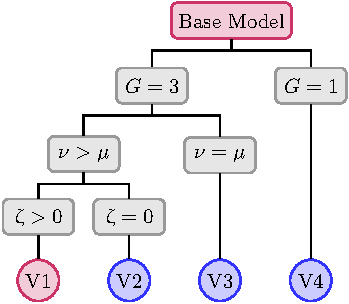
\includegraphics[width=0.7\linewidth]{variant-tree}
  \caption{Summary of the Full model (F) and three model variants (V)
    with respect to heterogeneity in risk, population growth (pop. growth), and turnover.
    Relative population size of each risk group is the same in all variants.
    $G$:~number of risk groups,
    $\nu$:~rate of population entry,
    $\mu$:~rate of population exit,
    $\phi$:~rates of population turnover.}
  \label{fig:variant-tree}
\end{figure}
\begin{table}
  \centering
  \caption{Parameters for model variants.}
  \label{tab:params-variants}
  \begin{threeparttable}
\begin{tabularx}{0.95\linewidth}{c *{4}{Y}}
	\toprule
	  Parameter    & Full                     & V1                           & V2                       & V3                                         \\
	\midrule
	$\bm{\hat{x}}$ & $[ 0.05\es0.20\es0.75 ]$ & ---                          & $[ 0.05\es0.20\es0.75 ]$ & $[ 0.05\es0.20\es0.75 ]$                   \\
	$\bm{\hat{e}}$ & $[ 0.05\es0.20\es0.75 ]$ & ---                          & $[ 0.05\es0.20\es0.75 ]$ & $[ 0.05\es0.20\es0.75 ]$                   \\
	     $C$       & $[ 25\es5\es1 ]$         & $[ \textbf{3} ]$\tnote{a}    & $[ 25\es5\es1 ]$         & $[ 25\es5\es1 ]$                           \\
	   $\delta$    & $[ 5\es15\es25 ]$        & $[ \textbf{33.3} ]$\tnote{b} & $[ 5\es15\es25 ]$        & $[ \textbf{33.3\es33.3\es33.3} ]$\tnote{b} \\
	    $\nu$      & $0.05$                   & $0.05$                       & $\textbf{0.03}$\tnote{c} & $0.05$                                     \\
	    $\mu$      & $0.03$                   & $0.03$                       & $0.03$                   & $0.03$                                     \\
	\bottomrule
\end{tabularx}
\footnotesize
\begin{tablenotes}
  \item
  $\bm{\hat{x}}$: proportion of individuals in the model by risk group (high, medium, low);
  $\bm{\hat{e}}$: proportion of individuals entering the model by risk group;
  $C$: rate of contact formation by risk group (per year);
  $\delta$: average duration in each risk group (years);
  $\nu$: rate of population entry (per year);
  $\mu$: rate of exit (per year).
  \item[a] Weighted average of risk-stratified $C$
  \item[b] Without turnover, duration in all groups must be equal to the inverse of the exit rate, $\mu^{-1}$
  \item[c] Adjusting the entry rate, versus exit rate, does not affect average duration in the model
\end{tablenotes}
\end{threeparttable}
\end{table}
% ==================================================================================================
\subsection{Influence of Rates of Turnover}\label{ss:exp-turnover}
To further examine the influence of turnover on
equilibrium prevalence and incidence,
we varied the rates of turnover in the Full model across a range of values.
We then conducted a sensitivity analysis
to examine the influence of turnover
at different treatment rates (durations of infectiousness).
% --------------------------------------------------------------------------------------------------
\paragraph{Experiment 2.1: Influence of the rates of turnover on equilibrium prevalence and incidence}
\label{p:exp-2-turnover-1}
%% SM: start by something like this to orient the reader and help with interpretation before results section
%% JK: I agree this could be useful, but then we go back-and forth between
%% implementation ("controlled by a single parameter") and
%% an overview of the experiment ("influence of turnover on ...")
%% I'd rather introduce how turnover is controlled via duration in high risk group
%% after noting why we cannot simply scale the rates proportionally with a single parameter.
In this experiment, we first considered the influence of turnover
at a fixed duration of infectiousness (treatment rate).
As in similar experiments \citep{Zhang2012,Henry2015},
the rates of turnover were scaled by a single parameter.
However, because the model used here has $G = 3$ risk groups,
multiplying by a set of base rates $\phi$ by a scalar factor
would have resulted in changes to the relative population size of risk groups $\bm{\hat{x}}$.
Thus, we controlled the rates of turnover by adjusting
the duration of individuals in the high risk group $\delta_H$,
such that a shorter period of time spent engaged in highest risk
corresponded to higher rates of turnover among all groups.
As in Experiment 1, we assumed that:
the proportion of individuals who enter each risk group $\bm{\hat{e}}$
is equal to
the proportion of individuals across risk groups in the model $\bm{\hat{x}}$;
and that the absolute number of individuals
moving between two groups in either direction is balanced.
The duration of individuals in the medium risk group $\delta_M$
was then defined as a value between $\delta_H$ and the maximum duration $\mu^{-1}$
which scales with $\delta_H$ following the equation:
$\delta_M = \delta_H + \kappa \left(\mu^{-1} - \delta_H\right)$, with $\kappa = 0.3$.
Finally, the duration of individuals in the low risk group $\delta_L$
similarly scaled with $\delta_H$,
but the value was not required to calculate $\phi$;
it can be determined from $\phi$ afterwards
using Eq.~(\ref{eq:duration-group}).
In this way, each value of $\delta_H$ was used to define a set of turnover rates $\phi$
whose elements all scaled inversely with the duration in the high risk group $\delta_H$.
The value of $\delta_H$ is then varied from 3~to~33 years to examine the influence of turnover.
% --------------------------------------------------------------------------------------------------
\paragraph{Experiment 2.2: Influence of the rates of turnover at various treatment rates}
\label{p:exp-2-turnover-2}
Next, we conducted a 2-way sensitivity analyses to examine how
the influence of turnover might vary at different treatment rates.
The treatment rate controls the duration of infectiousness $\delta_{\mathcal{I}}$
as in $\delta_{\mathcal{I}} = \tau^{-1}$.
Treatment rate $\tau$ was varied from 1~to~0.05,
implying a duration of infectiousness of 1~to~20 years.
The duration of time spent in the high risk group $\delta_H$
was varied from 3~to~33 years as in Experiment 2.1.
We examine the influence of the rates of turnover on
equilibrium prevalence and incidence across the
range of treatment rates using multiple 1D plots and 2D surface plots.
% ==================================================================================================
\subsection{Influence of turnover on the contribution of highest risk group to overall transmission}
\label{ss:exp-turnover-fit}
Finally, we examined the influence of turnover when fitting models to observed data
on disease prevalence across risk groups.
We use two models: the Full model with turnover, and model variant V3 without turnover
(Figure~\ref{fig:variant-tree}: F and V3).
Both models include population growth and 3 risk groups.
We then fit the following parameter in both models:
the contact rates among the highest and lowest risk groups, $C_H$ and $C_L$.
Specifically, we fit the models to equilibrium disease prevalence
in the highest and and lowest risk groups.
%% SM: does this get us the same overall (total population) prevalence?
%% JK: I never verified specifically, but I think so. I can check next iteration.
%Then, we infer the degree of risk heterogeneity in the population, as in $C_H / C_L$.
%% JK: re. commented out above: I think maybe this is too much repetition
%% with description in experiment 3.1
We then estimate the contribution of the highest risk group to overall transmission from both models.
The contribution is estimated as
the transmission population attributable fraction (TPAF)~\citep{Mishra2016}
of the highest risk group.
% --------------------------------------------------------------------------------------------------
\paragraph{Experiment 3.1: Influence of turnover on inferred risk heterogeneity}
%% SM: the part about comparing non-fitted scenarios does not come through here or in Experiment 3.2.
%% I wonder if that diagram we drew a long time ago on a whiteboard re: the comparisons could be helpful?
%% JK: I think mainly that is important for 3.2, as 3.1 is really only exploring
%% the inferred risk heterogeneity, which is relevant to fitting, but not really to non-fitted models.
%% What do you think?
The Full model (turnover) and model variant V3 (no~turnover) are calibrated to
25\% infection prevalence in the high risk group, and % SS: prevalence of infection; JK: clarified.
5\% in the low risk group at equilibrium.
%% SM: they should also reproduce overall prevalence too? what do you think?
%% JK: agree -- as above, I'll add this next iteration :) need to double check it is happening now.
The fitted parameters are
the contact rates of the high and low risk groups: $C_H$~and~$C_L$.%
\footnote{The fitted parameters are estimated by minimizing
  the negative log-likelihood of each predicted prevalence versus the target
  (assuming a sample size of 1000)
  using the Sequential Least SQuares Programming (SLSQP) method~\citep{Kraft1988}
  from the \texttt{scipy.optimize.minimize} Python package.}
The ratio of fitted (or posterior) contact rates $C_H~/~C_L$
represents the degree of risk heterogeneity in the population, after fixing all other parameters,
which produce the group-specific observed disease prevalence.
% --------------------------------------------------------------------------------------------------
\paragraph{Experiment 3.2: Influence of turnover on the predicted TPAF of the highest risk group}
We then calculate and compare the TPAF of the highest risk group
across the model variants with and without turnover.
We repeat this analysis using the default model parameters (before model fitting),
and again using the inferred values of $C_H$~and~$C_L$ (after model fitting).
%% SM: Suggest we put hypotheses in introduction
%% Thus, differences in inferred risk heterogeneity due to turnover from Experiment 3.1
%% are hypothesized to result in differences in the estimated TPAF of the high risk group.
%% JK: do you mean introduction to the paper, or introduction to this experiment (3)?
%% Leaving it out for now.